\section{Characteristic parameters}
The main method of stability testing is to check the values of multiple parameters in different runs and determine the abnormal runs by identifying the outliners. The most important characteristic parameters is the invariant mass distribution of all out-going particles. The other parameters, such as photon number recorded by different ECALs, are also used for the diagnosis of abnormalities.

\begin{figure*}[!ht]
	\centering
	\begin{subfigure}[b]{0.49\textwidth}
		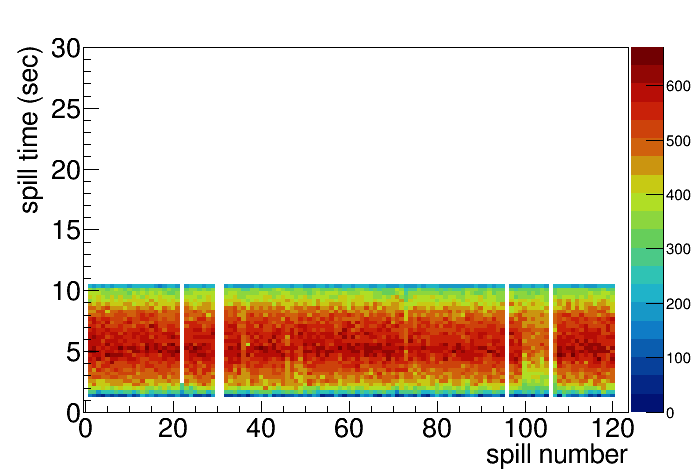
\includegraphics[width=\textwidth]{event_spill_70171}
		\caption{Run number 70171}
		\label{fig:EveN_spill_normal}
	\end{subfigure}
	~ %add desired spacing between images, e. g. ~, \quad, \qquad, \hfill etc. 
	%(or a blank line to force the subfigure onto a new line)
	\begin{subfigure}[b]{0.49\textwidth}
		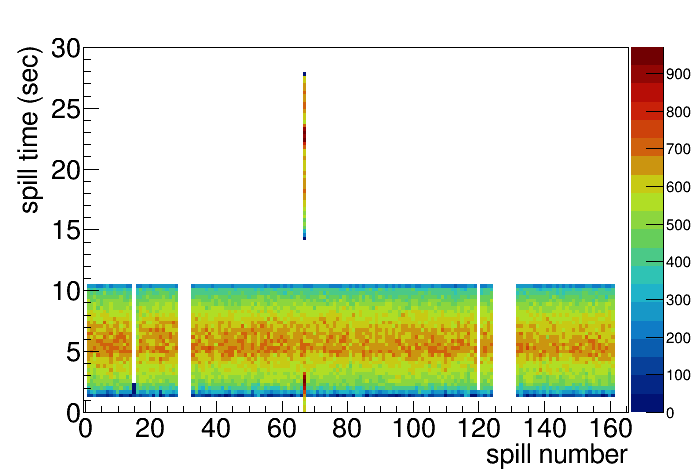
\includegraphics[width=\textwidth]{strange_spill_70195}
		\caption{Run number 70195}
		\label{fig:EveN_spill_abnormal}
	\end{subfigure}
	\caption{Temporal distribution of event numbers for each spill number. The color band represents the number of events per 0.3 seconds (time resolution) for each spill. The y axes represent the time from starting moment of each spill. (a) A normal temporal distribution (run number = 70171). The effective time expansion of particle beam is around 9s and distribution of each spill is centrally concentrated. (b) An abnormal temporal distribution (run number = 70195). Particle beam occurred in inactive time period.}
	\label{fig:animals}
\end{figure*}

\begin{figure*}[!h]
	\centering
	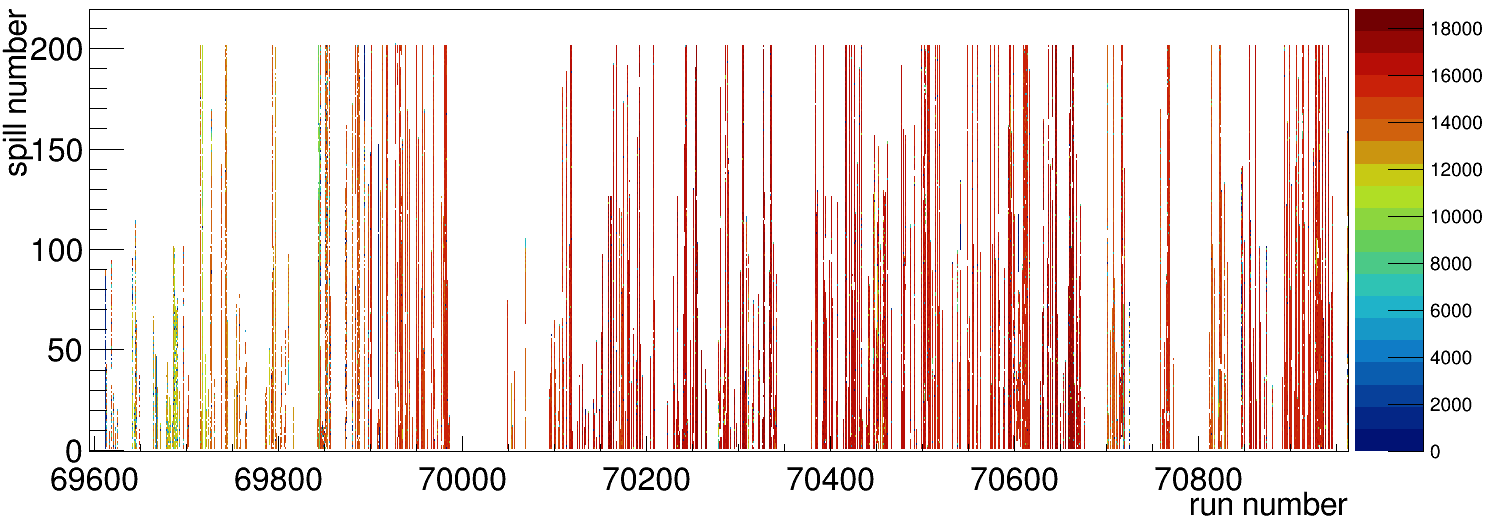
\includegraphics[width=\textwidth]{event_distribution_all}
	\caption{Event distribution with respect to spill number of each run number. The color band shows the value of event counting in certain spill of certain run. The run number ranging from $69595 \sim 70963$ while the maximal of spill number cannot exceed above 200. The number of events can goes up to 18000 per spill whereas it could also amount to only few thousands or less, especially in the beginning of experiment. }
	\label{fig:event_distribution_all}
\end{figure*}

\subsection{Number of events}
The number of events for each run can be vastly different after the preselection. By using PHAST data analysis framework, the event number for each spill of every run is counted and plotted. Since incoming particle beam only exist in certain time interval of spill, event numbers are not spread uniformly throughout the whole period of spill. From the figure \ref{fig:EveN_spill_normal}, one can easily see that, in normal case, events are only distributed on the time interval \SI{1.2}{\second} $\sim$ \SI{10.5}{\second} of the spill period. There is a short dead period of \SI{1.2}{\second} before the start of particle beam and a long inactive period after \SI{10.5}{\second} till the end of spill (at around \SI{48}{\second}). However, as is shown in figure \ref{fig:EveN_spill_abnormal}, there exists one abnormal run, where the effective time interval of one spill is more than 2 times larger than the normal one. To be exact, the particle beam occurs not only during the inactive time interval right at the beginning of spill (\SI{0}{\second} $\sim$ \SI{1.2}{\second}), but also after the first stop of beam (\SI{14.1}{\second} $\sim$ \SI{27.9}{\second}). Such abnormality could probably result from the trigger problem, due to which events are recorded with wrong time scale\footnote[2]{The abnormal run 70195 is ruled out at following analysis}.

After selecting out the run with abnormal temporal distribution discussed above, the number of events can be compared for each spill in every run, as is shown in figure \ref{fig:event_distribution_all}. The event number distribution is quite uneven throughout the experiment after the preselection. Runs in the beginning usually have low values of event counting and most of them don't have any event in some spills. Moreover, there even exist large number of vacant runs with no events in all spills. Therefore, one can consider the number of events of each run as the characteristic parameter to test the stability of experiment. However, analyses such as invariant mass of three pion mass are independent from the number of events one have for each run. Thus, the variation of event distribution throughout the experiment could have little or no effect towards results of the analyses.

\subsection{Vertex positions}
The next parameter that could be investigated is the position of vertices. The location of vertices cannot be measured directly from the detectors but rather reconstructed by the charged particle tracks. There are only two types of certice of each event extracted from PHAST: primary vertices and non-primary vertices. Generally, vertex position are determined by comparing out-going particle tracks and find the intercept point between two reconstructed tracks. If this intercept point also lies on the track of incoming particle, it is considered as a primary vertex. If not, it is considered as non-primary vertex. 

\begin{figure}[!b]
	\centering
	\begin{subfigure}[t]{0.5\textwidth}
		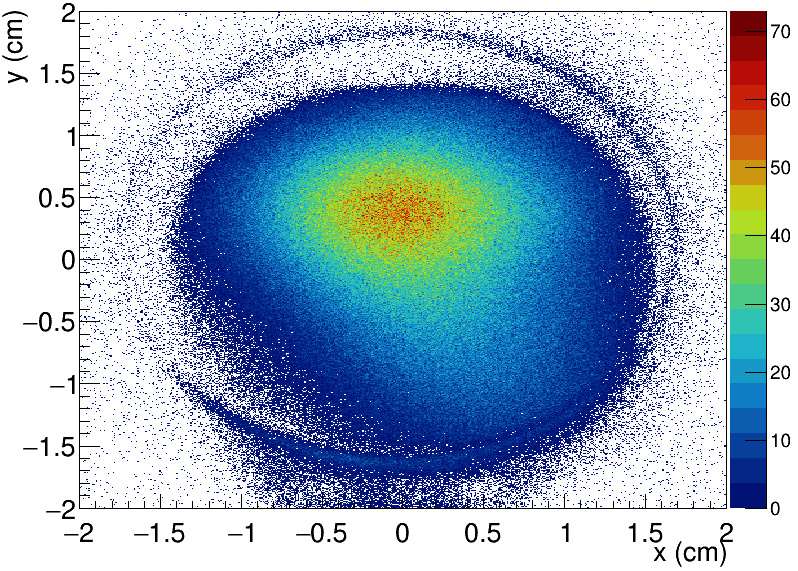
\includegraphics[width=\textwidth]{Prim_vertex_70171}
		\caption{Primary vertex positions}
		\label{fig:Prim_vertex_70171}
	\end{subfigure}
	~ %add desired spacing between images, e. g. ~, \quad, \qquad, \hfill etc. 
	%(or a blank line to force the subfigure onto a new line)
	\begin{subfigure}[b]{0.5\textwidth}
		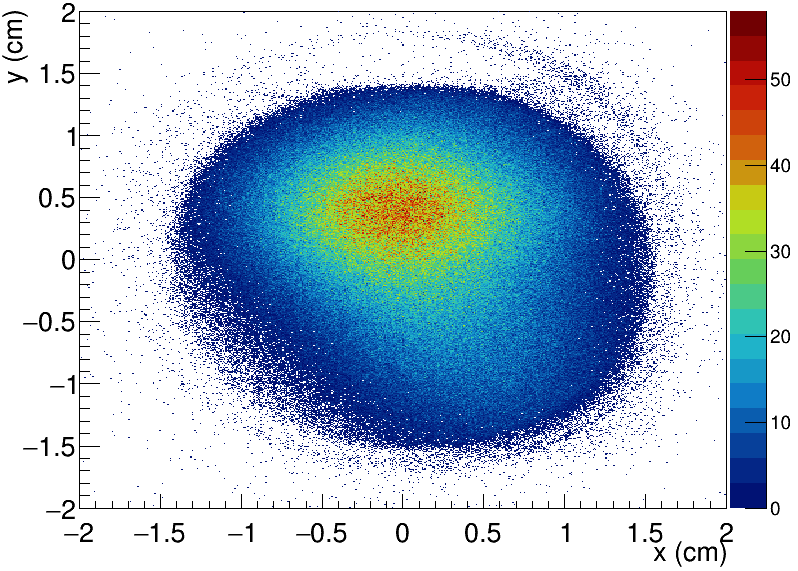
\includegraphics[width=\textwidth]{sec_vertex_70171}
		\caption{Non-primary vertex positions}
		\label{fig:sec_vertex_70171}
	\end{subfigure}
	\caption{vertex position distribution in x-y plane (z is the direction of the particle beam). The color band represents the number of vertices in corresponding location. Spacial resolution of x and y are both \SI{0.008}{\centi\meter}. (a) Distribution of primary vertices, in which a strange halo structure appears in the graph. (b) Distribution of non-primary vertices, where the halo disappears.}
	\label{fig:ver_pos}
\end{figure}

As has been discussed in subsection \ref{subsec:data_preselection}, the events after preselection contain either one charged track or three charged tracks. Event containing one charged track corresponds to elastic scattering while event with three charged tracks to inelastic scattering. In case of elastic scattering, since there is only one out-going particle track and one incoming particle track, all vertices being reconstructed are primary vertices. On the other hand, non-primary vertices could only exists in inelastic scattering. This can be better explained by vertices position map shown in figure \ref{fig:ver_pos}. The first graph, figure \ref{fig:Prim_vertex_70171}, shows the primary vertex position. As one can easily see, most of the vertex positions are on the liquid hydrogen target, which located at around $\SI{-1.4}{\centi\meter} \sim \SI{1.5}{\centi\meter}$ in x direction and $\SI{-1.5}{\centi\meter} \sim \SI{1.3}{\centi\meter}$ in y direction. Additional, there is halo shaped data points surrounding the target. The cause behind this strange shape is the elastic scattering between the $\pi$ beam and container of liquid hydrogen. From the vertices distribution on the center, one can see that the particle density of the beam is roughly Gaussian distributed in the cross section. In other words, there are more incoming particles in the central area of the beam than the peripheral area, leading to the decreasing of vertex density in the outward direction. But when the beam hits the metallic container, the vertex density surges due to the increase of elastic scattering cross-section between $\pi$ and metallic nucleus. Therefore, the vertices on the halo are most likely to be the primary vertices. This can be further proved when one checks the position of non-primary vertices. In figure \ref{fig:sec_vertex_70171}, the strange halo structure disappears, which indicates that most of events with three out-going particles corresponds to the inelastic scattering between the pion beam and hydrogen target.  

\subsection{Three pions invaraint mass}
The most obvious parameter that can be used for stability test should be the invariant mass distribution of three out-going pions, as is shown in figure \ref{fig:Three_pion_mass_his}. Since the total number of events in each run is significantly different, invariant mass distribution is normalized so that the maximal value of distribution is always equal to 1000. By such normalization, one can easily notice that positions of maximal value for each run are almost the same. If an individual run is extracted by doing the y projection of certain run number, the detailed structure of three pion invariant mass distribution can be obtained (see figure \ref{fig:Three_pion_mass_fitting}). The first peak locates around \SI{1.3}{\giga\electronvolt}, which is followed by a small second peak around \SI{1.67}{\giga\electronvolt} on the right side. To test its stability throughout the whole runs, position of first peak is calculated by fitting the graph with following function:
\begin{equation}
f(x) = a_0 \cdot \Big(\mathcal{N}(a_1, a_2^2)+a_3 \cdot \mathcal{N}(a_4, a_5^2)\Big)
\end{equation}
where $\mathcal{N}(\mu,\sigma^2)$ represents the Gaussian distribution with mean value $\mu$ and standard deviation $\sigma$. $a_0$, $a_1$, $a_2$, $a_3$, $a_4$ and $a_5$ are six fitting parameters with initial values: $a_0 \sim$ maximal value, $a_1 \sim 1$, $a_2 \sim 1$, $a_3 \sim 0.01$ and $a_5 \sim 1$. Through trails and errors, $a_4$ is fixed to be 1.49 to optimize the fitting curve for first peak.

\begin{figure*}[!ht]
	\centering
	\vspace{2cm}
	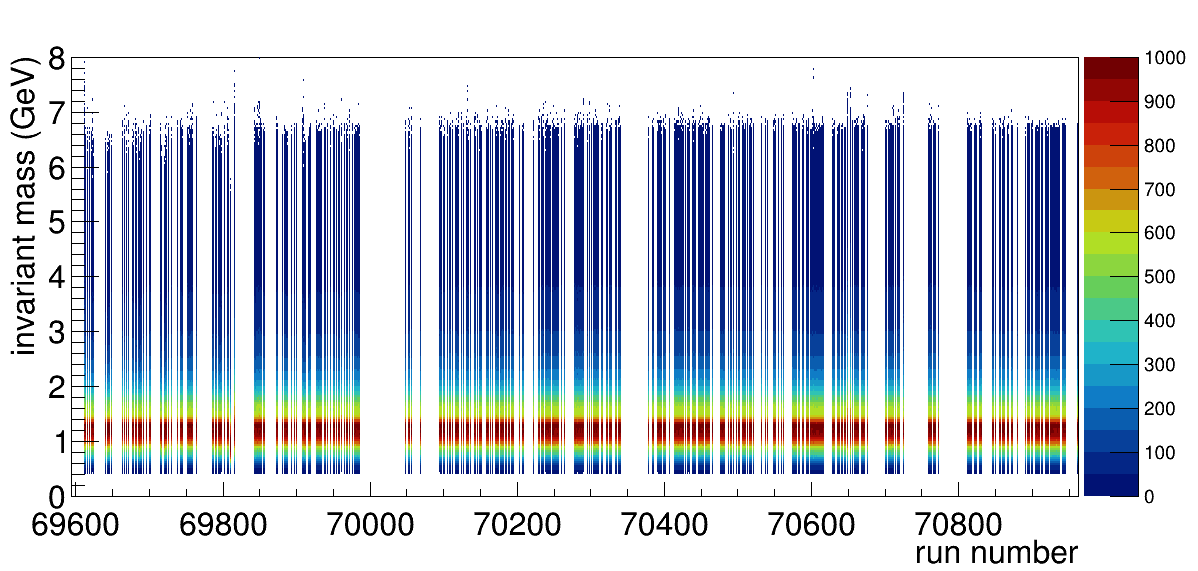
\includegraphics[width=\textwidth]{Three_pion_mass_his}
	\caption{Histogram of invariant mass distribution of three pions for each run. The colors inside the histogram represent number of events corresponding to run number and invariant mass. To better compare and conceive the structure of distribution between runs visually, the maximal value of each distribution is normalized to 1000. As one can easily notice that maximal value or peak of distribution locates around \SI{1.3}{\giga\electronvolt} for almost every run.}
	\label{fig:Three_pion_mass_his}
	\vspace{2 cm}
	
	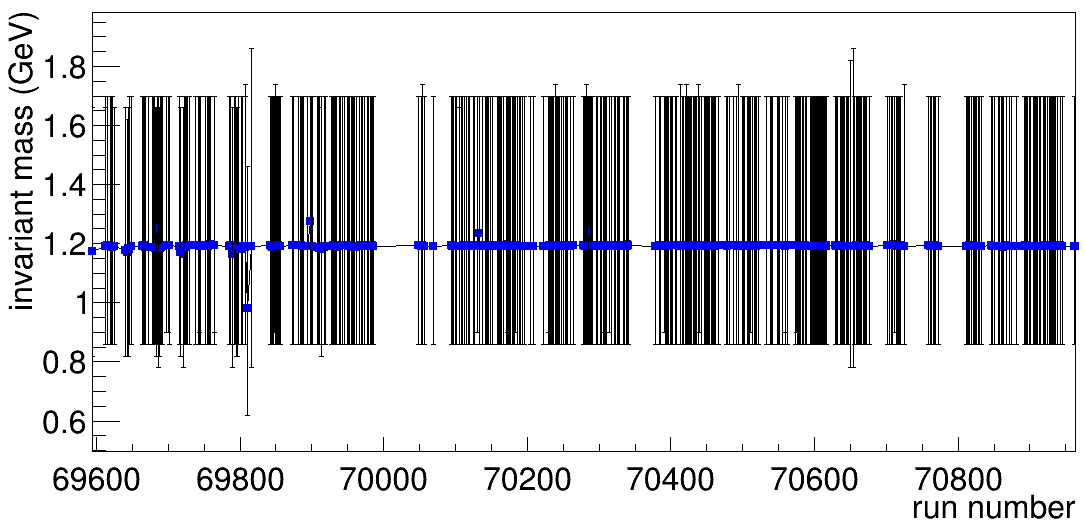
\includegraphics[width=\textwidth]{Three_pion_mass_Graph}
	\caption{Comparison of primary peak position and half maximum from each run. The blue dots shows the value of fitting parameter $a_1$, which correspond to positions of primary peak. The error bar the range of half maximum. An abnormal run with run number equal to 69811 (denoted in red circle) can be easily spotted in this plot.}
	\label{fig:Three_pion_mass_Graph}
	\vspace{2cm}
\end{figure*}

\begin{figure*}[t!]
	\centering
	\begin{subfigure}{0.48\textwidth}
		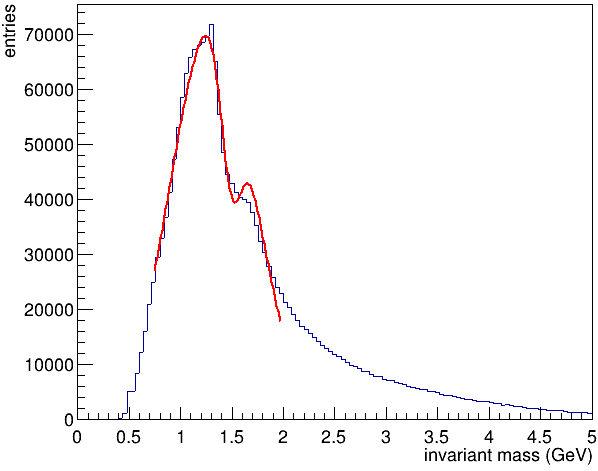
\includegraphics[width=\textwidth]{Three_pion_mass_fitting}
		\caption{run number 70171}
		\label{fig:Three_pion_mass_fitting}
	\end{subfigure}
	\begin{subfigure}{0.48\textwidth}
		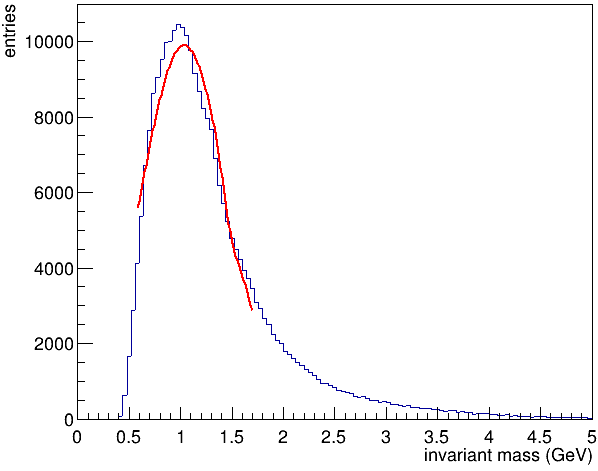
\includegraphics[width=\textwidth]{Three_pion_mass_69811}
		\caption{run number 69811}
		\label{fig:Three_pion_mass_69811}
	\end{subfigure}
	\caption{Invariant mass distribution of three pions and their corresponding fitting result. The range of fitting corresponds to \SI{30}{\percent} of maximal value of distribution. (a) Distribution of a normal run. The first peak (primary) locates at around \SI{1.3}{\giga\electronvolt}. The fitting curve (red) coincide well with data around primary peak, but poorly around second peak. (b) Distribution of an abnormal run. No second peak can be found on the right side of primary peak. Parameter $a_1$ is fitted to be \SI{1.034}{\giga\electronvolt}, which is slightly larger than correct value due to the bad fitting coincidence. }
	\label{fig:pion_mass}
\end{figure*}



The fitting curve of a typical distribution is shown as the red curve in figure \ref{fig:Three_pion_mass_fitting}. The position of primary peak is represented by the value of $a_1$, which is fitted to be \SI{1.305}{\giga\electronvolt}. Figure \ref{fig:Three_pion_mass_Graph} shows the result after carrying out such fitting to each run and calculated the position value of primary peak as well as range of half maximum of corresponding distribution. One outliner can be easily identified (in red circle of figure \ref{fig:Three_pion_mass_Graph}) with the run number equal to 69811. Figure \ref{fig:Three_pion_mass_69811} shows its corresponding distribution. It is not hard to discover that for run 69811, not only there exists no noticeable second peak but also its primary peak shifts a little to the left side, which results in a smaller value shown in figure \ref{fig:Three_pion_mass_Graph}.
\subsection{Total invariant mass}
The next parameter worth investigating is the invariant mass of all out-going particles, a.k.a out-going pions and photons. The four-momentum of pions can be obtained as in the same way as in previous subsection. To obtain the four-momentum of photons, energy cuts are applied differently to two electromagnetic calorimeters (ECAL) and remaining photons are all assumed to come from primary vertex.
\subsubsection{Photon energy cut}
\begin{figure}[!t]
	\centering
	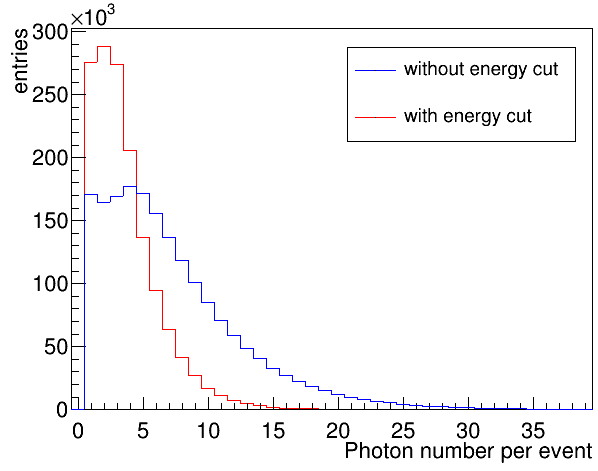
\includegraphics[width=0.5\textwidth]{photon_energy_cut}
	\caption{Effect of energy cut of photons. On the x axis is the number of photons captured by both ECALS and on the y axis shows the number of events (entries) which have corresponding photon numbers. Blue line is the histogram of events without photon energy cut and red line events with photon energy cut. As can be seen easily that number of events with small number of photons are increased significantly after energy cut.}
	\label{fig:photon_energy_cut}
\end{figure}
As has been discussed in subsection \ref{subsec:photon}, photons can also be emitted during the interaction. Different from the charged pions, which can leave tracks in tracking detector via ionization, photon has no charge and no track can be found. The only way to identify photons is by its energy deposits in ECAL. However, ECAL can only gives the energy of each photon and the direction of its momentum cannot be determined by any detectors in COMPASS experiment. Thus, the vertex which photon comes from cannot be determined neither. On the other hand, photons captured by ECALs could also come from the background instead of scattering vertex. Photons from background are mainly generated by bremsstrahlung between beam particles or outgoing pions and the material of detectors. Nevertheless, those background photons usually have a very small energy compared to those coming out of scattering vertices. Thus, to differentiate the photons from scattering vertices and photons from background, energy cuts are applied on the data coming from each calorimeter. Considering photons only coming from the scattering, since the photons detected by first ECAL (ECAL1) has larger scattering angle than those by ECAL2, energy deposits on the ECAL1 are generally smaller than on the ECAL2. Thus the energy cut for ECAL1 should be smaller than the cut for ECAL2, as is shown by following:

\begin{center}
	\begin{tabular}{c||c}
		Calorimeter & Energy cut      \\
		\hline
		ECAL1       & \textgreater{}\SI{1}{\giga\electronvolt} \\
		\hline
		ECAL2       & \textgreater{}\SI{4}{\giga\electronvolt}
	\end{tabular}
\end{center}



Photons with energy smaller than energy cut are selected out on both ECALs. The result of energy cut is shown in figure \ref{fig:photon_energy_cut}. As one can easily notice that, without energy cut, there are sufficient amount of events that could have more than 10 photons in totally detected by calorimeters, which is highly unlikely in scattering process. Once energy cuts are applied and photons with low energy being removed, almost all events have only less than 10 photons. Assuming all photons after energy cuts come from the primary vertex, 4-momentum of each photon can, thus, be obtained.
\subsubsection{Total invariant mass}
\begin{figure}[!b]
	\centering
	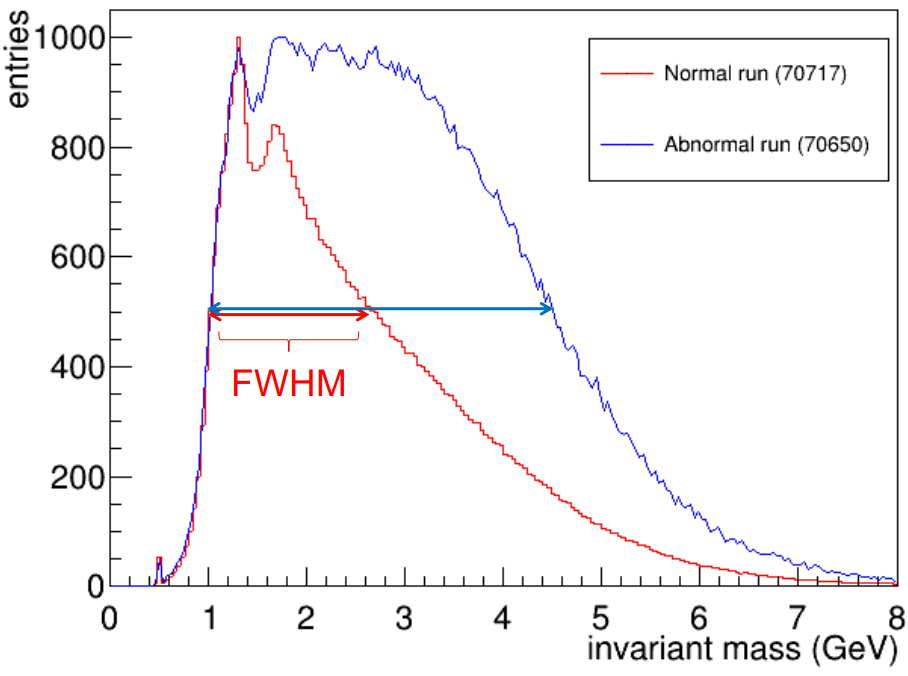
\includegraphics[width=0.5\textwidth]{Total_mass_comp}
	\caption{Comparison of normalized total invariant mass distribution between normal run and abnormal run. Both maximal value of both distribution are set to be 1000. On the x axis shows the value of total invariant mass and on the y axis shows the entries of corresponding value. FWHM is width of the range between two points, which corresponds to 500 value. As can be seen very clearly that the abnormal run (70650) has a much larger FWHM value than the normal run (70717).}
	\label{fig:Total_mass_comp}
\end{figure}
Total invariant mass is a very important parameter, from which the mass of intermediate unknown resonance state X (in figure \ref{fig:feymann_diag}) can be calculated. If for each run, the physics in scattering process is same, total invariant mass should also be very stable. Figure \ref{fig:Total_mass_his} shows the normalized invariant mass distribution for each run. For most of runs, the maximal entries locate between around \SI{1}{\giga\electronvolt} to \SI{2}{\giga\electronvolt}. However, as can be already noticed in this 2 dimensional histograms, there are several runs which have much longer range of high entries (shown in red boxes). The detailed distribution structure of an normal run (run number 70717) is shown in figure \ref{fig:Total_mass_comp} (red line), compared with the structure from one of abnormal runs (run number 70650, blue line). One can immediately see that for abnormal run, it has a much bigger full width half maximal (FWHM) value than normal run. Both runs have first peak in same position. But for abnormal run, the entry value does not go down immediately after the place of second peak. To examine this phenomenon throughout the whole experiment, FWHM value is calculated for each run and drawn in figure \ref{fig:Total_mass_FWHM}. For most of runs, the values concentrate on the range between around \SI{1.4}{\giga\electronvolt} to \SI{1.8}{\giga\electronvolt}. But there also exist some outliners with much larger FWHM value up to \SI{3.5}{\giga\electronvolt}. On the other hand, some runs have slight smaller value, ranging from \SI{1.3}{\giga\electronvolt} to \SI{1.4}{\giga\electronvolt}.

There are two possibilities resulting in this abnormal phenomenon. One is related to abnormality during the process of scattering. The other is related to the malfunction of calorimeters since the number of abnormal runs concerning total invariant mass is larger than the case of three pion invariant mass. The first could be checked directly by the recoil proton ($p'$ in figure \ref{fig:feymann_diag}).

\begin{figure*}[!ht]
	\centering
	\vspace{2cm}
	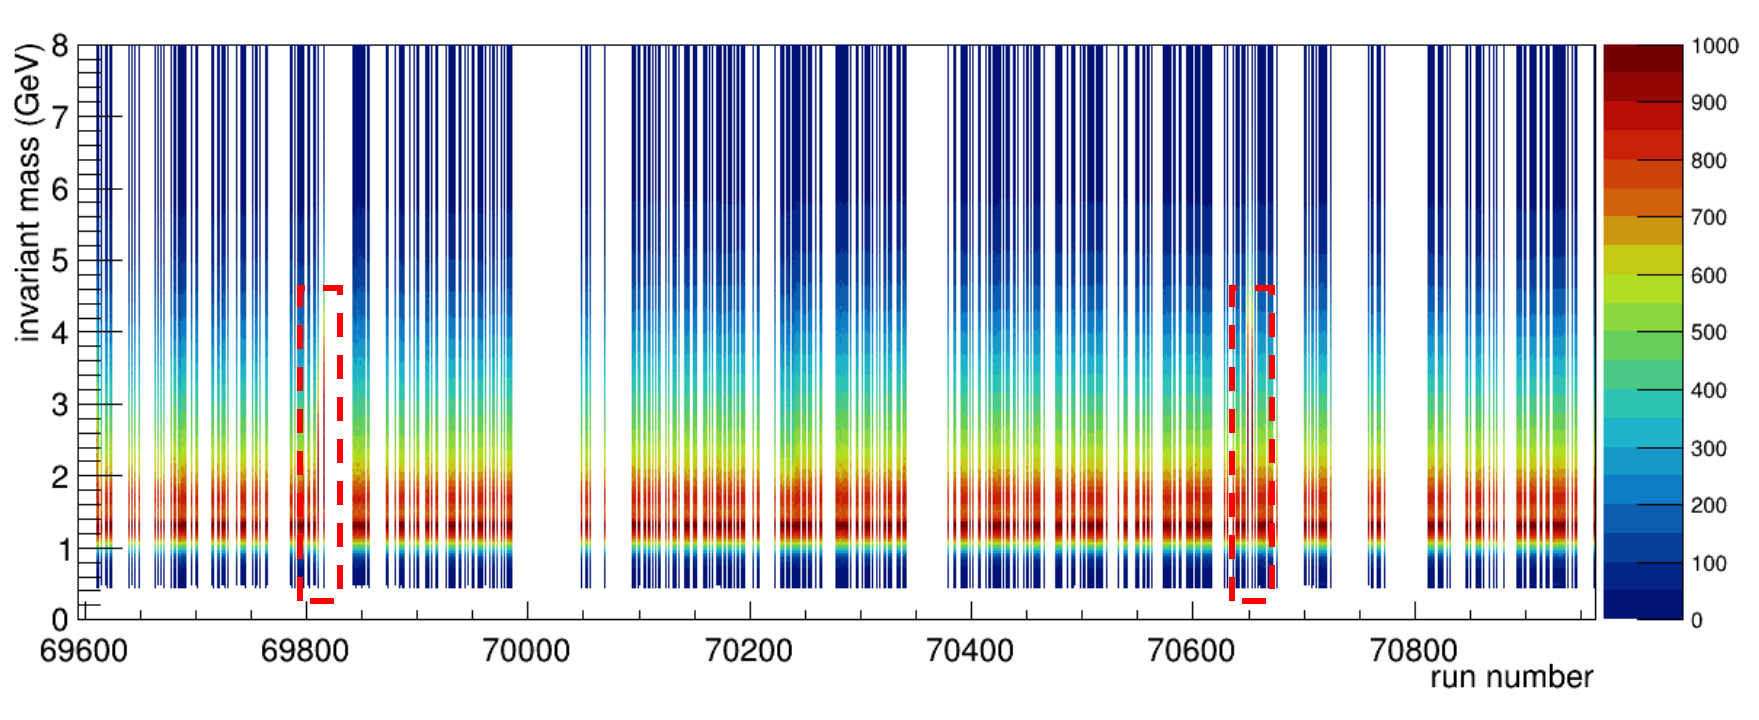
\includegraphics[width=\textwidth]{Total_mass_his}
	\caption{Histogram of invariant total mass distribution. The colors inside the histogram represent number of events corresponding to the run number and invariant mass. To better compare and conceive the structure of distribution between runs visually, the maximal value of each distribution is normalized to 1000. In the red dashed rectangles, it can be seen that the red strokes are much longer than the normal runs.}
	\label{fig:Total_mass_his}
	\vspace{2 cm}
	
	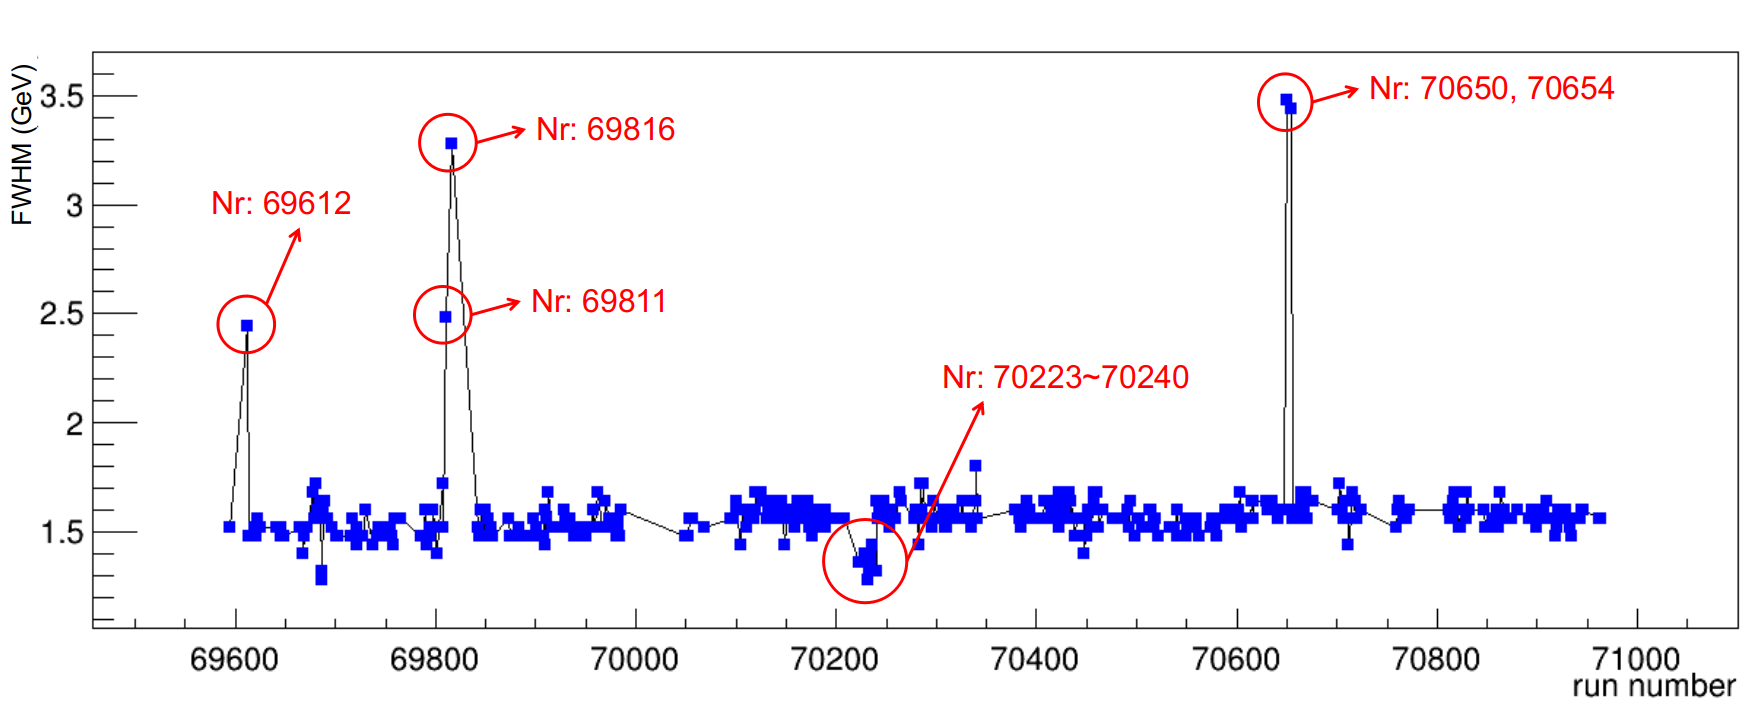
\includegraphics[width=\textwidth]{Total_mass_FWHM}
	\caption{Value of full width at half maximum of total invariant distribution for each run. Typical value of FWHM for normal run is around \SI{1.5}{\giga\electronvolt}.There are several outliners that have much bigger FWHM value than the general one. Also there is a range of runs 70223 $\sim$ 70240 that have slight smaller value of FWHM. }
	\label{fig:Total_mass_FWHM}
	\vspace{3cm}
\end{figure*}

\subsection{Recoil proton}

\label{subsec:recoil_proton}
As has been discussed in subsection \ref{subsec:Detector_layout} and depicted in figure \ref{fig:sandwich}, recoil-proton detector is in cylindrical shape, surrounding the liquid hydrogen target. Any proton knocked out of the target would be directly detected by RPD. Unfortunately, same as for calorimeters, RPD can also not measure the momentum of captured protons but their energy. Thus, the vertex of recoil proton is assumed to be the primary vertex of the event. The scattering angle of recoil proton can be further calculated from capturing position on RPD and its corresponding primary vertex. Angular distribution of recoil proton is shown in figure \ref{fig:Recoil_proton_comp}. For both runs, the distributions peak at around $\theta=\SI{1.35}{\radian} = 77.35^{\circ}$, where $\theta$ is angle between the z direction of beam and momentum direction of out-going proton. The disparities between normal run and abnormal are shown in the lower half of the distribution. As for the abnormal run, a huge bump occurs on the left side of peak below \SI{45}{\percent} of maximal value, which can be reflected numerically by calculating the width of certain height, such as \SI{23}{\percent} of maximal value.

\begin{figure}[!b]
	\centering
	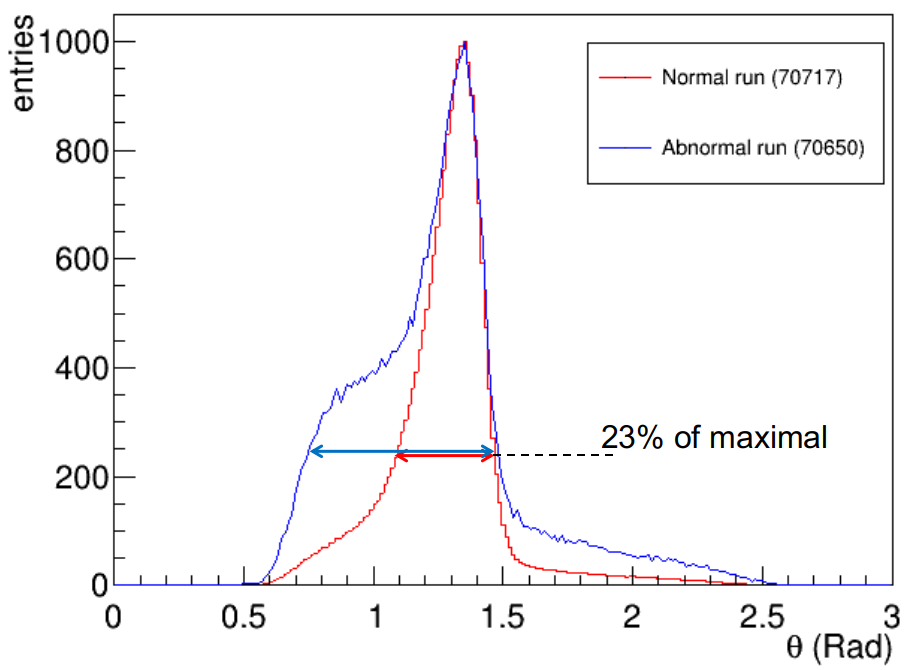
\includegraphics[width=0.5\textwidth]{Recoil_proton_comp}
	\caption{Normalized angular distribution of recoil proton. On the x axis is $\theta$, which is the polar angle of out-going proton with respect to z direction of particle beam. Y axis shows the entries of events with the corresponding scattering angle. Red curve represents of a normal distribution from run number equal to 70717 and blue curve is an abnormal distribution from run number 70650. Both are normalized so that the maximal values are 1000. At \SI{23}{\percent} of maximal value (randomly chosen), two runs have significant value of width. }
	\label{fig:Recoil_proton_comp}
\end{figure}

\begin{figure}[!b]
	\centering
	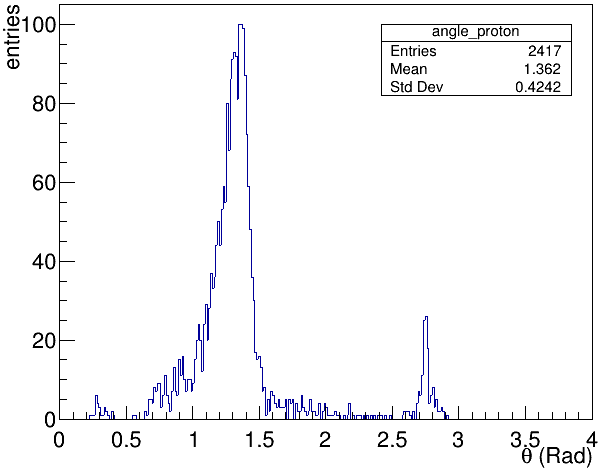
\includegraphics[width=0.5\textwidth]{Recoil_proton_double_peak}
	\caption{Angular distribution of recoil proton with run number equal to 70054. On the right side of primary peak occurs another small peak, which corresponds to situation that protons are recoiled nearly in the opposite direction of incoming pion beam. }
	\label{fig:Recoil_proton_double_peak}
\end{figure}

\begin{figure*}[!h]
	\centering
	\vspace{1cm}
	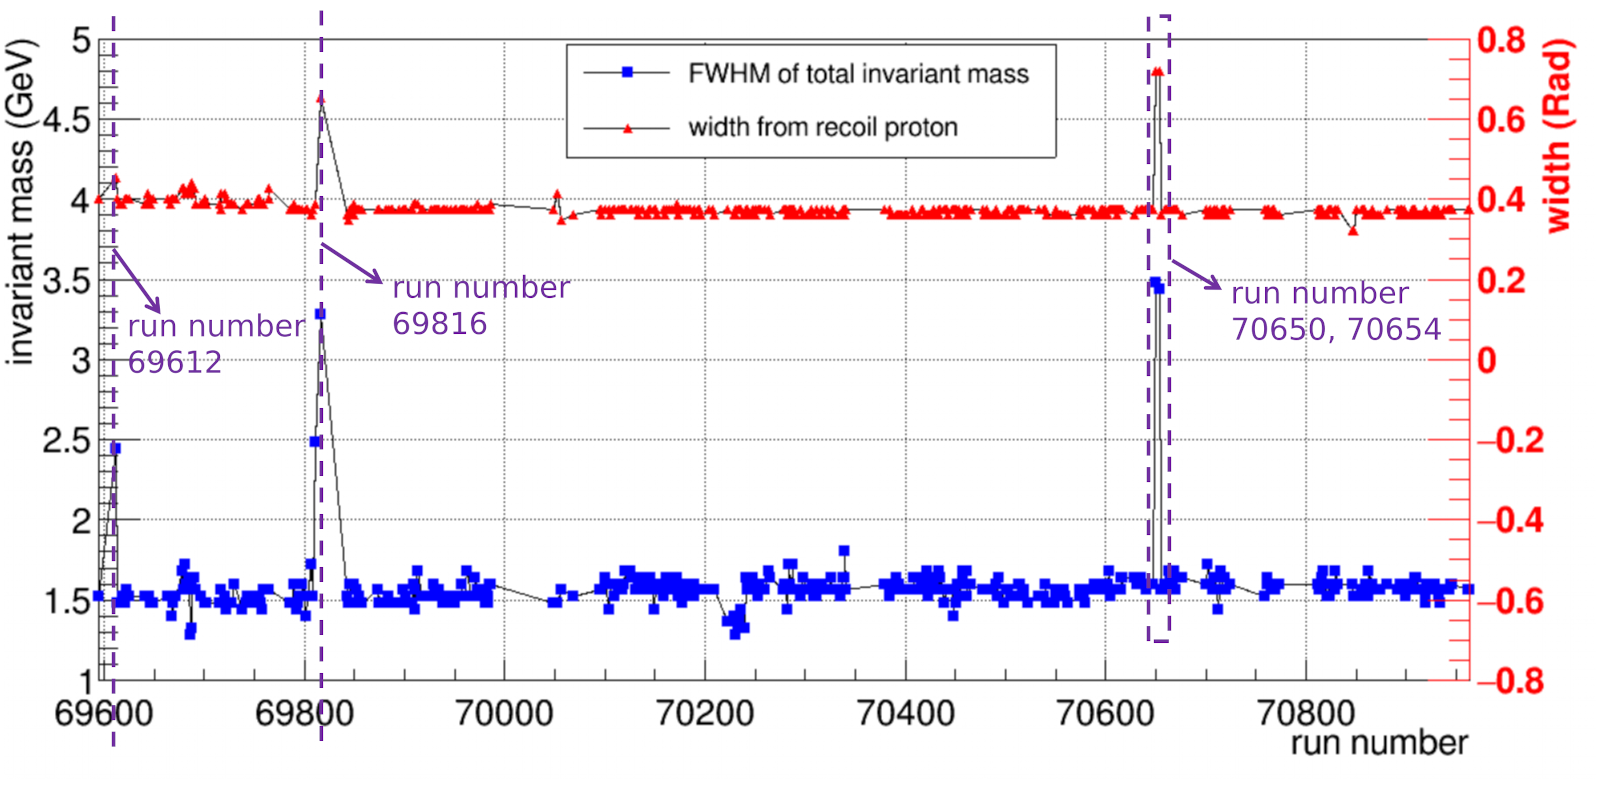
\includegraphics[width=\textwidth]{Total_mass_recoil_proton}
	\caption{Comparison between the FWHM value of total invariant mass (blue) and the width (at 23\% of maximal value) of angular distribution of recoil proton (red). On the right vertical axis are the values of recoil proton width and on the left are the values of invariant mass. Three regions can be found for the evidence of correlation: 69612, 69816 and 70650$\sim$70654. All the abnormal runs are positive correlated between these two parameters.}
	\label{fig:Total_mass_recoil_proton}
	\vspace{1 cm}
	
	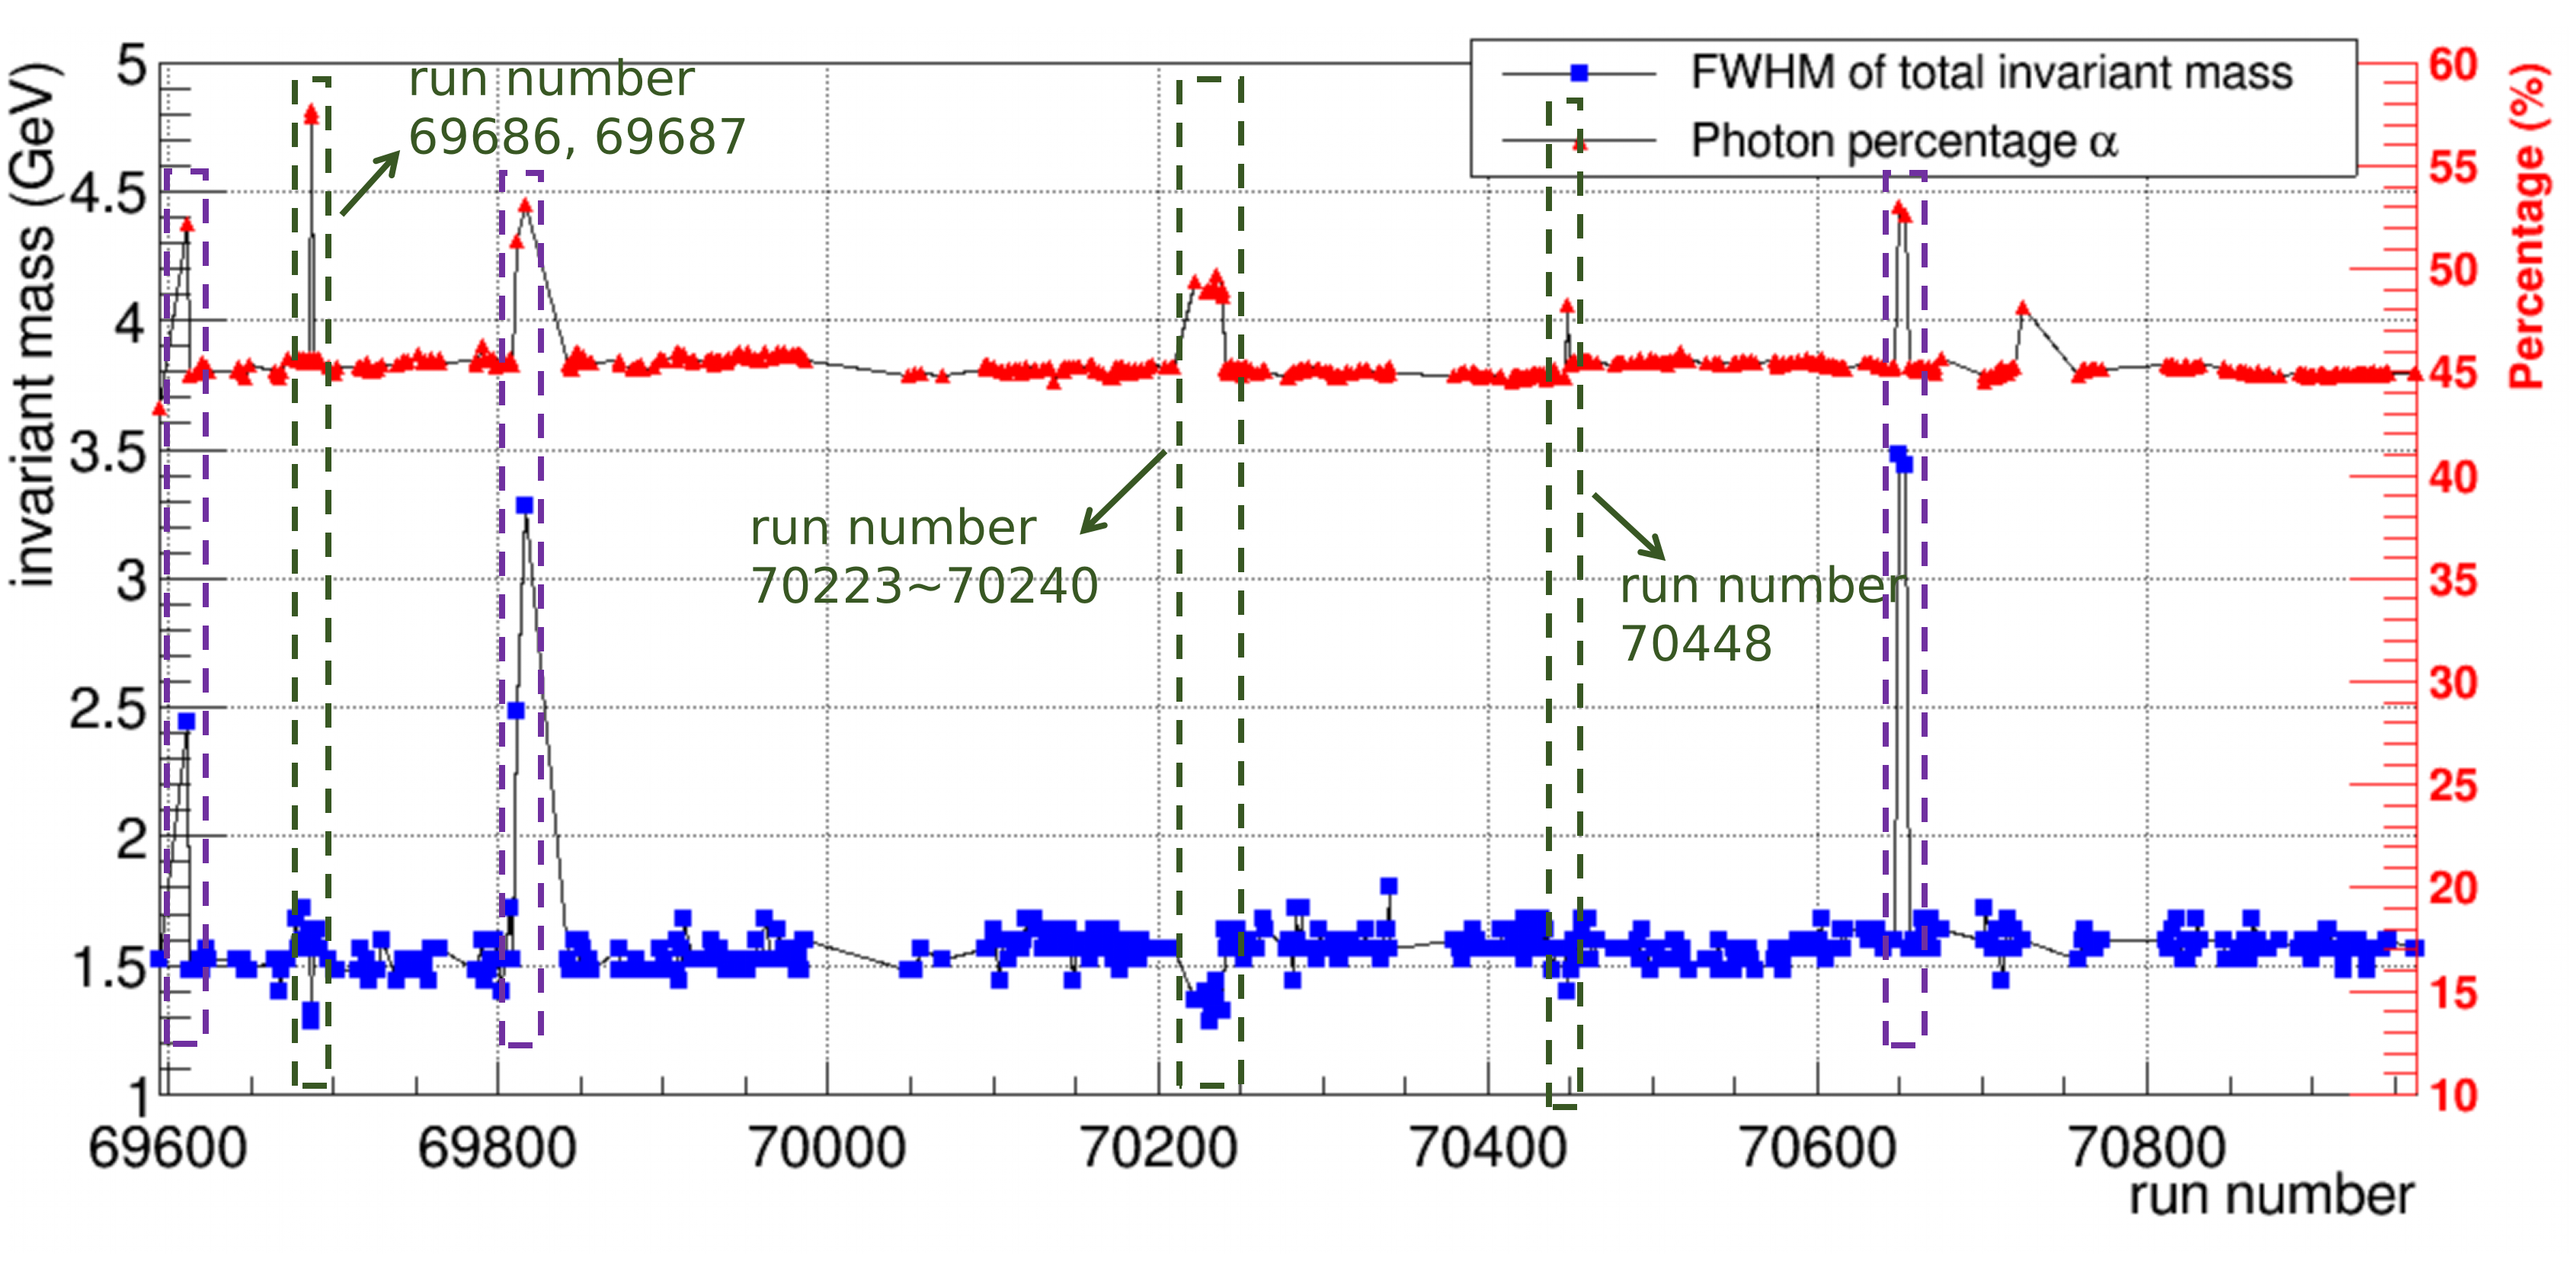
\includegraphics[width=\textwidth]{Total_mass_ECAL}
	\caption{Comparison between the FWHM value of total invariant mass (blue) and the photon number percentage $\alpha$ of calorimeters (red). For the normal runs, $\alpha$, the percentage of ECAL1, is around value of $45\%$. Apart from the positive correlated region (purple boxes) which has already existed in recoil proton width, there are three more negative correlated regions (green boxes): 69686$\sim$69687, 70223$\sim$70240 and 70448. Additionaly, the negative correlated regions only have a smaller deviation value than positive correlated regions.}
	\label{fig:Total_mass_ECAL}
	\vspace{1cm}
\end{figure*}

\begin{figure*}[!h]
	\centering
	\vspace{1cm}
	\begin{subfigure}{\textwidth}
		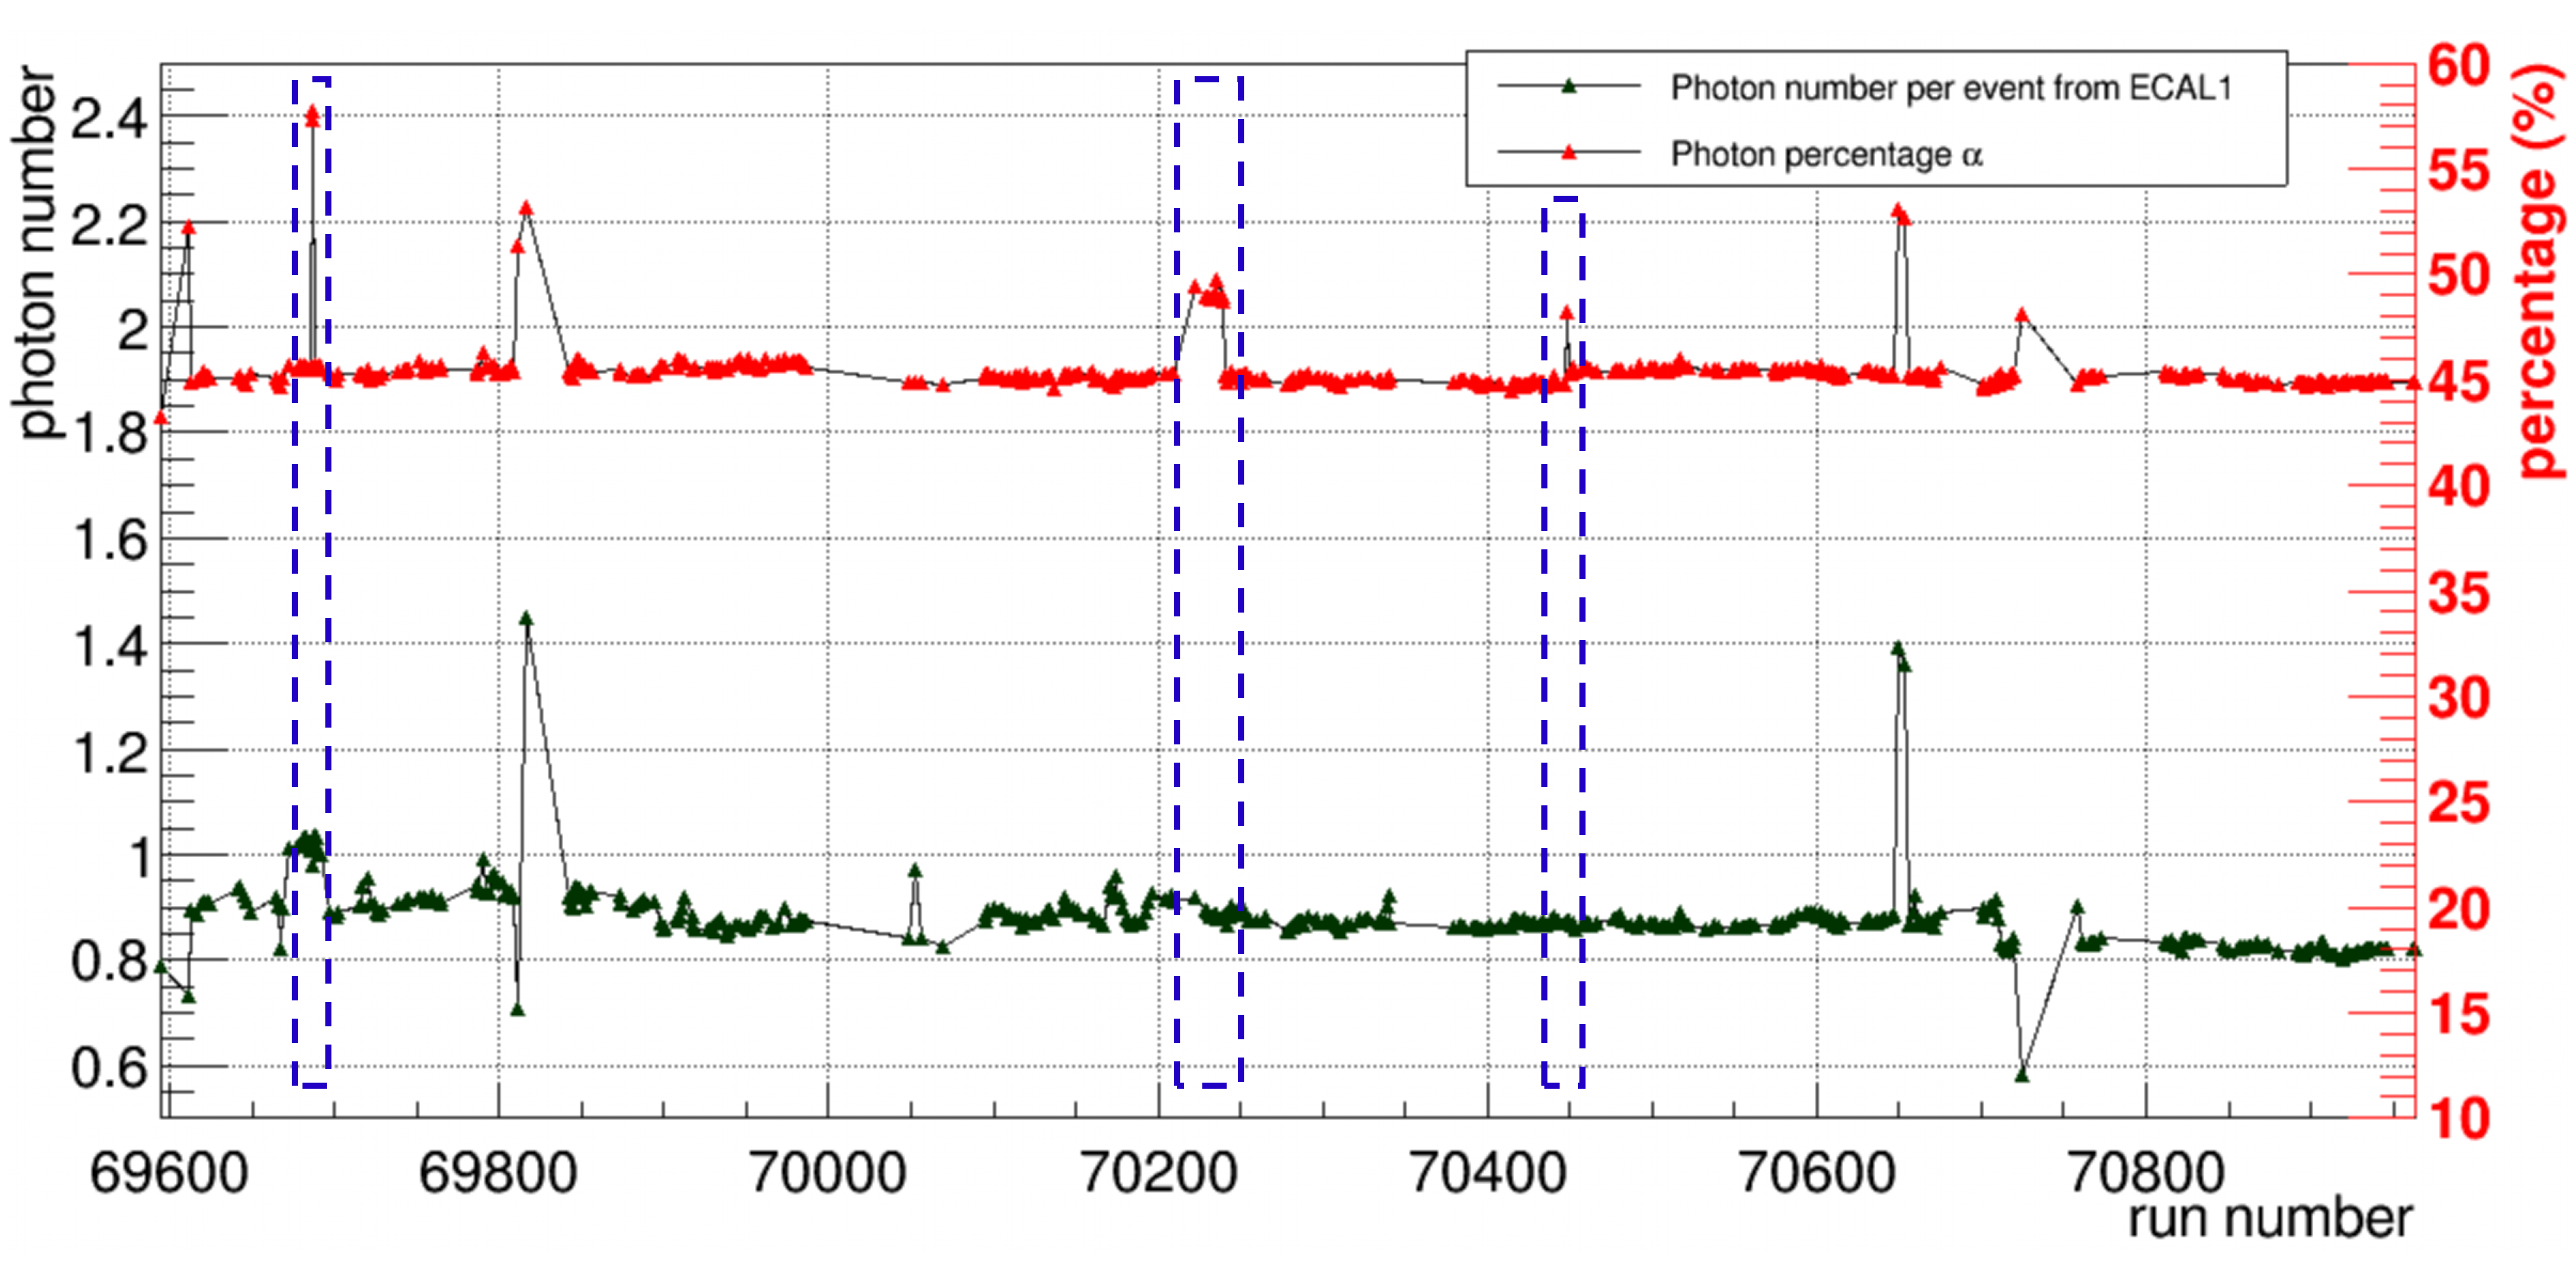
\includegraphics[width=\textwidth]{ECAL_per_ECAL1}
		\caption{ECAL1}
		\label{fig:ECAL_per_ECAL1}
		\vspace{1cm}
	\end{subfigure}
	\begin{subfigure}{\textwidth}
		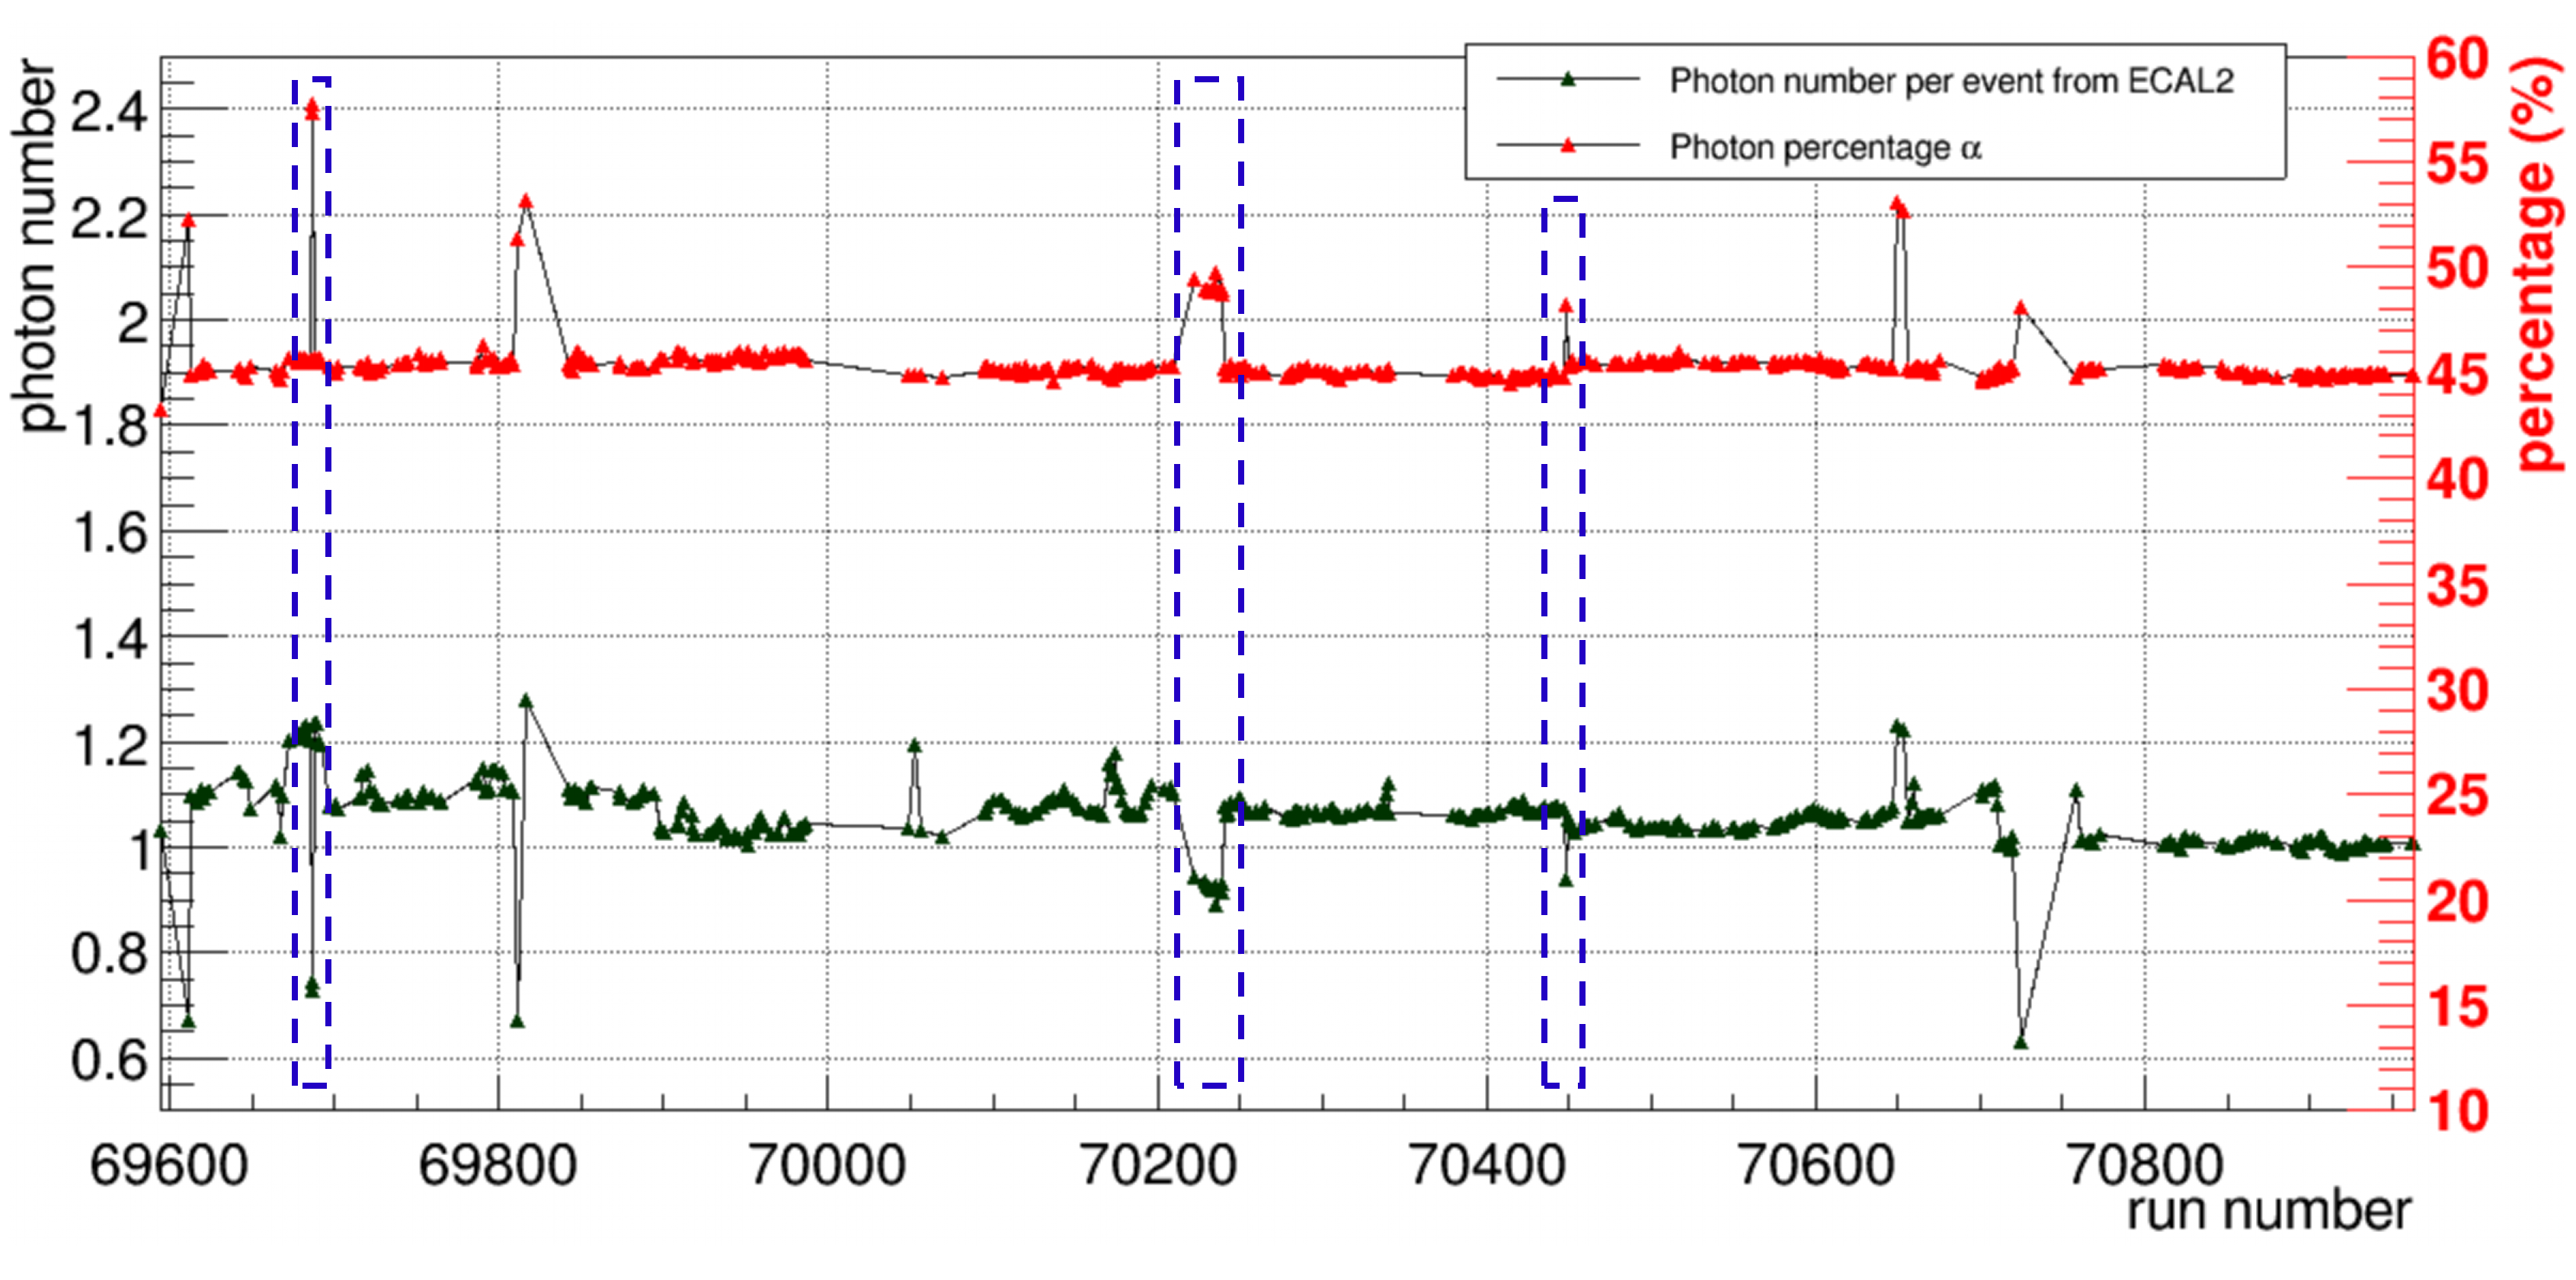
\includegraphics[width=\textwidth]{ECAL_per_ECAL2}
		\caption{ECAL2}
		\label{fig:ECAL_per_ECAL2}
	\end{subfigure}
	\caption{Detailed investigation of variation of $\alpha$, the photon number percentage of ECAL1. Averaged photon numbers for both two ECALs are calculated by dividing the total number of photon by the corresponding number of events in each run. Three negative correlated regions are shown by purple boxes. (a) comparison between the $\alpha$ (red) and photon number per event from ECAL1 (green). No abnormality appears in correlated regions for ECAL1. (b) comparison between the $\alpha$ (red) and photon number per event from ECAL2 (green). Declines of ECAL2 photon number are found in all negative correlated regions.}
	\label{fig:ECAL_per_ECAL}
	\vspace{1cm}
\end{figure*}

The second type of abnormality (run number 70054) is shown in figure \ref{fig:Recoil_proton_double_peak}, where another peak occurs at the range $\SI{2.7}{\radian} \sim \SI{2.8}{\radian}$. Theoretically speaking, the scattering angle $\theta$ cannot be larger than $\pi/2$ for recoil proton since it cannot be hit backwards by the incoming pions. In the real case, the reconstruction of out-going particle tracks causes the uncertainty of primary vertex position and, thus, errors on scattering angle $\theta$. This is the reason why even for a normal run, it also contains small amount of events with proton being recoiled at angles slightly bigger than $\pi/2$. But for run number 70054, there are events where the recoil angles reach to $\SI{2.7}{\radian}$. One of explanations of this phenomenon is defect of triggers. Due to this recoil proton absorbed by RPD does not come from the primary vertex in its corresponding event and the false recoil angle is calculated. Therefore, the runs with such abnormality should be ruled out during analysis.





